\documentclass[11pt]{article}

\usepackage{tikz, pgfplots}
\usepackage{circuitikz}
\usetikzlibrary{shapes,arrows,fit,calc,positioning,decorations}
\usetikzlibrary{shadows,arrows}
% Define the layers to draw the diagram
\pgfdeclarelayer{background}
\pgfdeclarelayer{foreground}
\pgfsetlayers{background,main,foreground}
 
% Define block styles  
\tikzstyle{materia}=[draw, fill=white, text width=6.0em, text centered,
  minimum height=1.5em,drop shadow]
\tikzstyle{practica} = [materia, text width=8em, minimum width=10em,
  minimum height=3em, rounded corners, drop shadow]
\tikzstyle{texto} = [above, text width=20em, right]
\tikzstyle{linepart} = [draw, thick, color=black!50, -latex', dashed]
\tikzstyle{line} = [draw, thick, color=black!50, -latex']
\tikzstyle{ur}=[draw, text centered, minimum height=0.01em]
 
% Define distances for bordering
\newcommand{\blockdist}{1.3}
\newcommand{\edgedist}{1.5}

\newcommand{\practica}[2]{node (p#1) [practica]
  {#2}}

% Draw background
\newcommand{\background}[5]{%
  \begin{pgfonlayer}{background}
    % Left-top corner of the background rectangle
    \path (#1.west |- #2.north)+(-0.8,0.8) node (a1) {};
    % Right-bottom corner of the background rectanle
    \path (#3.east |- #4.south)+(+0.8,-0.5) node (a2) {};
    % Draw the background
    \path[fill=gray!20,rounded corners, draw=black!50, dashed]
      (a1) rectangle (a2);
    \path (a1.east |- a1.south)+(1.2,-0.2) node (u1)[texto]
      {\scriptsize\hspace{-12mm}\textit{#5}};
  \end{pgfonlayer}}

\newcommand{\transreceptor}[3]{%
  \path [linepart] (#1.east) -- node [above]
    {\scriptsize Transreceptor #2} (#3);}

\begin{document}

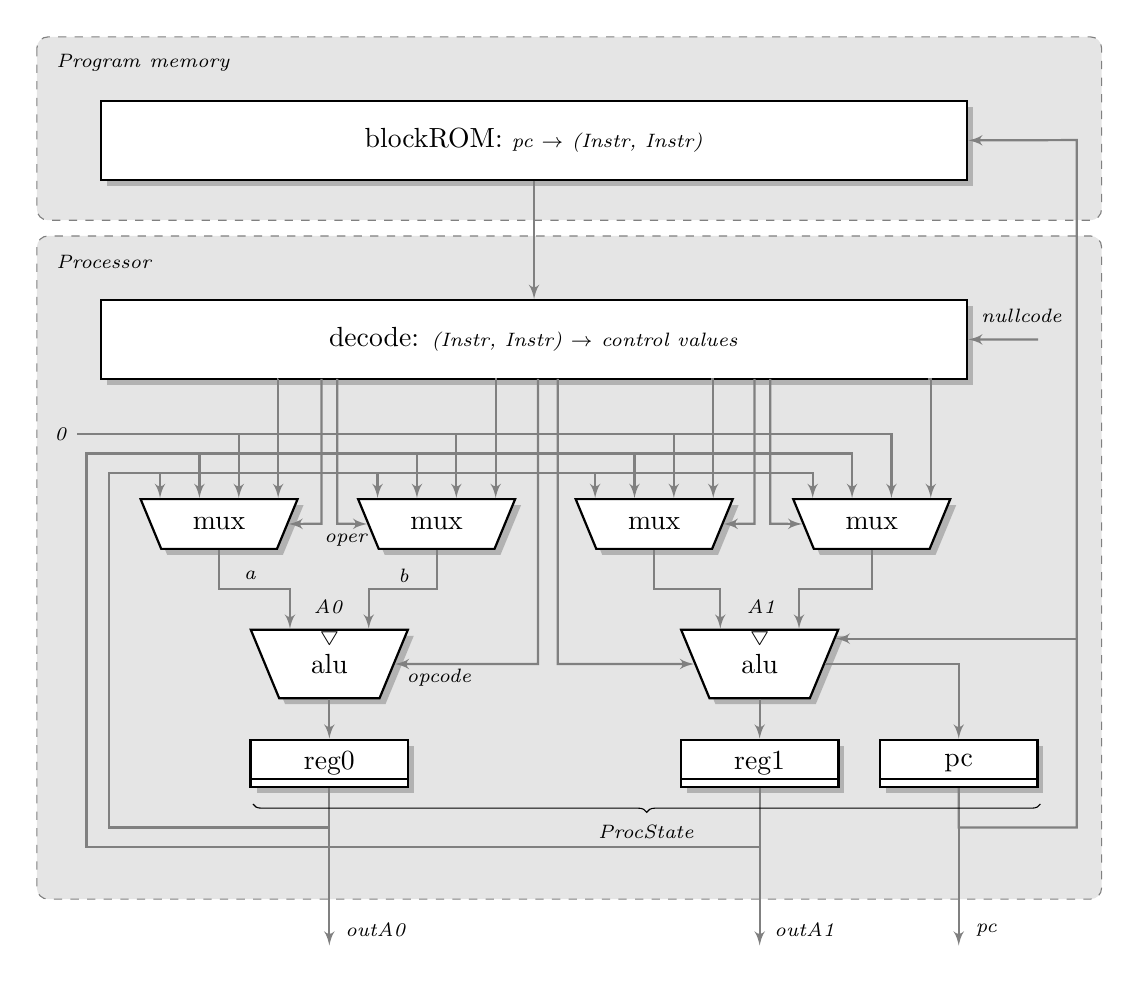
\begin{tikzpicture}[thick]
\tikzset{input/.style={}}
\tikzset{block/.style={rectangle,draw,fill=white,drop shadow}}
\tikzset{block2/.style={rectangle,draw}}
\tikzset{nop/.style={rectangle}}
\tikzstyle{pinstyle} = [pin edge={to-,thick,black}]
\tikzset{mux/.style={trapezium, trapezium angle=-67.5, draw, drop shadow, fill=white}}

\node [block, input, xshift=1.5 cm, yshift=-1.5 cm, minimum width=11cm, minimum height=1cm] (de) {decode: \scriptsize \textit {(Instr, Instr) $\rightarrow$ control values}};
\node [block, above=1.5 cm of de, minimum width=11cm, minimum height=1cm] (br) {blockROM: \scriptsize \textit {pc $\rightarrow$ (Instr, Instr)}};
\draw[line] (br.south) -- (de.north);

\node [mux, below=1.5 cm of de, minimum width=2cm, minimum height=0.6cm, xshift=-4 cm] (m1) {mux};
\node [mux, right=1 cm of m1,   minimum width=2cm, minimum height=0.5cm] (m2) {mux};
\node [mux, right=1 cm of m2,   minimum width=2cm, minimum height=0.5cm] (m3) {mux};
\node [mux, right=1 cm of m3,   minimum width=2cm, minimum height=0.5cm] (m4) {mux};

\node [mux, below=1 cm of m1, minimum width=2cm, minimum height=0.5cm, xshift=1.4 cm] (a0) {alu};
\node [mux, right=3.8 cm of a0, minimum width=2cm, minimum height=0.5cm] (a1) {alu};
\node[draw=none, yshift=-0.1cm] at (a0.north) {\scriptsize \textit {$\bigtriangledown$}};
\node[draw=none, yshift=-0.1cm] at (a1.north) {\scriptsize \textit {$\bigtriangledown$}};

\node [block,  below=0.5 cm of a0, minimum width=2cm, minimum height=0.6cm] (r0) {reg0};
\node [block2, below=0.5 cm of a0, minimum width=2cm, minimum height=0.5cm] (t1) {};
\node [block,  below=0.5 cm of a1, minimum width=2cm, minimum height=0.6cm] (r1) {reg1};
\node [block2, below=0.5 cm of a1, minimum width=2cm, minimum height=0.5cm] (t1) {};
\node [block,  right=0.5 cm of r1, minimum width=2cm, minimum height=0.6cm] (pc) {pc};
\node [block2, right=0.5 cm of t1, minimum width=2cm, minimum height=0.5cm] (t2) {};

\path [line] (m1.south) -| +(0,-0.5) -| ([xshift=-0.5 cm]a0.north);
\path [line] (m2.south) -| +(0,-0.5) -| ([xshift=0.5 cm]a0.north);
\path [line] (m3.south) -| +(0,-0.5) -| ([xshift=-0.5 cm]a1.north);
\path [line] (m4.south) -| +(0,-0.5) -| ([xshift=0.5 cm]a1.north);

\path [line] (a0.south) -| (r0.north);
\path [line] (a1.south) -| (r1.north);

\path [line] (r0.south) -| +(0,-2) node[anchor=west] {\scriptsize \textit {}};
\path [line] (r1.south) -| +(0,-2) node[anchor=west] {\scriptsize \textit {}};
\path [line] (pc.south) -| +(0,-2) node[anchor=west] {\scriptsize \textit {}};
\node[draw=none, xshift=-0.5cm, yshift=-9cm] at (0,0) {\scriptsize \textit {outA0}};
\node[draw=none, xshift=4.95cm, yshift=-9cm] at (0,0) {\scriptsize \textit {outA1}};
\node[draw=none, xshift=7.25cm, yshift=-9cm] at (0,0) {\scriptsize \textit {pc}};

\path [line] (r0.south) -| +(0,-0.5) -| +(-2.8,4) -| ([xshift=-0.75 cm]m1.north);
\path [line] (r0.south) -| +(0,-0.5) -| +(-2.8,4) -| ([xshift=-0.75 cm]m2.north);
\path [line] (r0.south) -| +(0,-0.5) -| +(-2.8,4) -| ([xshift=-0.75 cm]m3.north);
\path [line] (r0.south) -| +(0,-0.5) -| +(-2.8,4) -| ([xshift=-0.75 cm]m4.north);

\path [line] (r1.south) -| +(0,-0.75) -| +(-8.55,4.25) -| ([xshift=-0.25 cm]m1.north);
\path [line] (r1.south) -| +(0,-0.75) -| +(-8.55,4.25) -| ([xshift=-0.25 cm]m2.north);
\path [line] (r1.south) -| +(0,-0.75) -| +(-8.55,4.25) -| ([xshift=-0.25 cm]m3.north);
\path [line] (r1.south) -| +(0,-0.75) -| +(-8.55,4.25) -| ([xshift=-0.25 cm]m4.north);

\path[line] +(-1.2,-2) -| +(-1.2,-3.84) -- +(m1.east) ;
\path[line] +(-1,-2)   -| +(-1,-3.84)   -- +(m2.west) ;
\path[line] +(4.3,-2)  -| +(4.3,-3.84)  -- +(m3.east) ;
\path[line] +(4.5,-2)  -| +(4.5,-3.84)  -- +(m4.west) ;

\path[line] +(1.55,-2) -| +(1.55,-5.623) -- +(a0.east) ;
\path[line] +(1.8,-2)  -| +(1.8,-5.623)  -- +(a1.west) ;

\path [line] (-4,-2.7)   -| ([xshift=0.25 cm]m1.north);
\path [line] (-4,-2.7)   -| ([xshift=0.25 cm]m2.north);
\path [line] (-4,-2.7)   -| ([xshift=0.25 cm]m3.north);
\path [line] (-4.3,-2.7) -| ([xshift=0.25 cm]m4.north);
\node[draw=none, yshift=-0.1cm] at (-4.5,-2.6) {\scriptsize \textit {0}};

\path [line] (-1.75,-2) -| ([xshift=0.75 cm]m1.north);
\path [line] (1,-2)     -| ([xshift=0.75 cm]m2.north);
\path [line] (3.75,-2)  -| ([xshift=0.75 cm]m3.north);
\path [line] (6.5,-2)   -| ([xshift=0.75 cm]m4.north);

\path [line] (a1.east)   -| (pc.north);
\path [line] (8.4,-5.3) -- +(-3.07,0);
\path [line] (pc.south)  -| +(0,-0.5) -| +(1.5,8.23) -- (br.east);
\path [line] (7.9, -1.5)   -- (de.east);

\node[draw=none, xshift=7.7cm, yshift=-1.2cm] at (0,0) {\scriptsize \textit {nullcode}};
\node[draw=none, xshift=-1.1cm, yshift=-4.9cm] at (0,0) {\scriptsize \textit {A0}};
\node[draw=none, xshift=4.4cm, yshift=-4.9cm] at (0,0) {\scriptsize \textit {A1}};
\node[draw=none, xshift=0.3cm, yshift=-5.8cm] at (0,0) {\scriptsize \textit {opcode}};
\node[draw=none, xshift=-2.1cm, yshift=-4.5cm] at (0,0) {\scriptsize \textit {a}};
\node[draw=none, xshift=-0.15cm, yshift=-4.5cm] at (0,0) {\scriptsize \textit {b}};
\node[draw=none, xshift=-0.88cm, yshift=-4.05cm] at (0,0) {\scriptsize \textit {oper}};

%left,top,right,bottom
\node [nop, below=0.01 cm of a1, minimum width=3cm, minimum height=2cm] (n) {};
\background{de}{de}{pc}{n}{Processor};
\background{de}{br}{pc}{br}{Program memory};

\draw [decorate,decoration={brace,amplitude=3pt},xshift=3.93cm,yshift=-9.4cm]
(4,2) -- (-6,2) node[midway, font=\footnotesize, yshift=-10pt] {\scriptsize \textit {ProcState}};
\end{tikzpicture}

\end{document} 
